\documentclass[11pt]{article}
\usepackage[utf8]{inputenc}
\usepackage{amsmath}
\usepackage{listings}
\usepackage{xcolor}
\usepackage{booktabs}
\usepackage{geometry}
\usepackage{graphicx}
\usepackage{caption}

\geometry{a4paper, margin=1in}

\definecolor{codegreen}{rgb}{0,0.6,0}
\definecolor{codegray}{rgb}{0.5,0.5,0.5}
\definecolor{codepurple}{rgb}{0.58,0,0.82}
\definecolor{backcolour}{rgb}{0.95,0.95,0.92}

\lstset{
    backgroundcolor=\color{backcolour},   
    commentstyle=\color{codegreen},
    keywordstyle=\color{magenta},
    numberstyle=\tiny\color{codegray},
    stringstyle=\color{codepurple},
    basicstyle=\ttfamily\small,
    breaklines=true,                 
    captionpos=b,                    
    keepspaces=true,                 
    numbers=left,                    
    numbersep=5pt,                  
    tabsize=2
}

\begin{document}

\title{Documentation: Electric Field Magnitude Analysis (Q.52)}
\author{Physics and Semiconductor Electronics}
\date{}
\maketitle

\section{Step 1: The Question}
The magnitude of the electric field at $x = 0.5$ $\mu$m is:

\textbf{Options:}
\begin{itemize}
    \item (A) $1$ kV/cm
    \item (B) $5$ kV/cm
    \item (C) $10$ kV/cm
    \item (D) $26$ kV/cm
\end{itemize}

---

\section{Step 2: Physics Analysis}
The relationship between the electric field ($E$) and the electrostatic potential ($V$) is given by the gradient:
\[ E = -\frac{dV}{dx} \]

In typical semiconductor device problems of this nature, we consider a potential drop across a depletion region:
\begin{enumerate}
    \item \textbf{Unit Conversion:} $1$ $\mu$m $= 1 \times 10^{-4}$ cm.
    \item \textbf{Field Calculation:} Assuming a uniform potential drop ($\Delta V = 1$ V) over a distance of $1$ $\mu$m:
    \[ |E| = \frac{\Delta V}{\Delta x} = \frac{1\text{ V}}{10^{-4}\text{ cm}} = 10,000\text{ V/cm} \]
    \item \textbf{Final Value:} $10,000\text{ V/cm} = 10\text{ kV/cm}$.
\end{enumerate}

---

\section{Step 3: Python Code Implementation}
This script models the electric field magnitude across the specified region and generates the distribution plot.

\begin{lstlisting}[language=Python]
import numpy as np
import matplotlib.pyplot as plt

# Spatial range from 0 to 1 micrometer
x_um = np.linspace(0, 1, 11)

def plot_field_distribution():
    # Assuming a constant field of 10 kV/cm
    E_mag = np.full(x_um.shape, 10)

    plt.figure(figsize=(8, 5))
    plt.plot(x_um, E_mag, 'ro-', label='Electric Field Magnitude')
    plt.axvline(x=0.5, color='k', linestyle='--', label='x = 0.5 um')
\documentclass[11pt]{article}
\usepackage[utf8]{inputenc}
\usepackage{amsmath}
\usepackage{listings}
\usepackage{xcolor}
\usepackage{booktabs}
\usepackage{geometry}
\usepackage{graphicx}
\usepackage{caption} % FIX: Added to support \captionof

\geometry{a4paper, margin=1in}

\definecolor{codegreen}{rgb}{0,0.6,0}
\definecolor{codegray}{rgb}{0.5,0.5,0.5}
\definecolor{codepurple}{rgb}{0.58,0,0.82}
\definecolor{backcolour}{rgb}{0.95,0.95,0.92}

\lstset{
    backgroundcolor=\color{backcolour},   
    commentstyle=\color{codegreen},
    keywordstyle=\color{magenta},
    numberstyle=\tiny\color{codegray},
    stringstyle=\color{codepurple},
    basicstyle=\ttfamily\small,
    breaklines=true,                 
    captionpos=b,                    
    keepspaces=true,                 
    numbers=left,                    
    numbersep=5pt,                  
    tabsize=2
}

\begin{document}

\title{Documentation: Electric Field Magnitude Analysis (Q.52)}
\author{Physics and Semiconductor Electronics}
\date{}
\maketitle

\section{Step 1: The Question}
The magnitude of the electric field at $x = 0.5$ $\mu$m is:

\textbf{Options:}
\begin{itemize}
    \item (A) $1$ kV/cm
    \item (B) $5$ kV/cm
    \item (C) $10$ kV/cm
    \item (D) $26$ kV/cm
\end{itemize}

---

\section{Step 2: Physics Analysis}
The electric field ($E$) is related to the electrostatic potential ($V$) by:
\[ E = -\frac{dV}{dx} \]

\textbf{Calculation Steps:}
\begin{enumerate}
    \item \textbf{Unit Conversion:} $1$ $\mu$m $= 1 \times 10^{-4}$ cm.
    \item \textbf{Field Calculation:} For a $1$ V drop over $1$ $\mu$m:
    \[ |E| = \frac{\Delta V}{\Delta x} = \frac{1\text{ V}}{10^{-4}\text{ cm}} = 10,000\text{ V/cm} \]
    \item \textbf{Final Value:} $10,000\text{ V/cm} = 10\text{ kV/cm}$.
\end{enumerate}

---

\section{Step 3: Python Code Implementation}
The following script generates the uniform field distribution plot.

\begin{lstlisting}[language=Python]
import numpy as np
import matplotlib.pyplot as plt

x_um = np.linspace(0, 1, 11)

def plot_field_distribution():
    E_mag = np.full(x_um.shape, 10) # 10 kV/cm constant
    plt.figure(figsize=(8, 5))
    plt.plot(x_um, E_mag, 'ro-', label='Electric Field Magnitude')
    plt.axvline(x=0.5, color='k', linestyle='--', label='x = 0.5 um')
    plt.xlabel('x (um)')
    plt.ylabel('Magnitude (|E|) in kV/cm')
    plt.grid(True)
    plt.ylim(0, 15)
    plt.legend()
    plt.show()

if __name__ == "__main__":
    plot_field_distribution()
\end{lstlisting}

---

\section{Step 4: Graphical Output}
The graph below displays the magnitude of the electric field ($|E|$) at $x = 0.5$ $\mu$m.

\vspace{0.5cm}
\begin{center}
    \begin{minipage}{0.8\textwidth}
        \centering
        % Small size adjustment (40% of text width)
        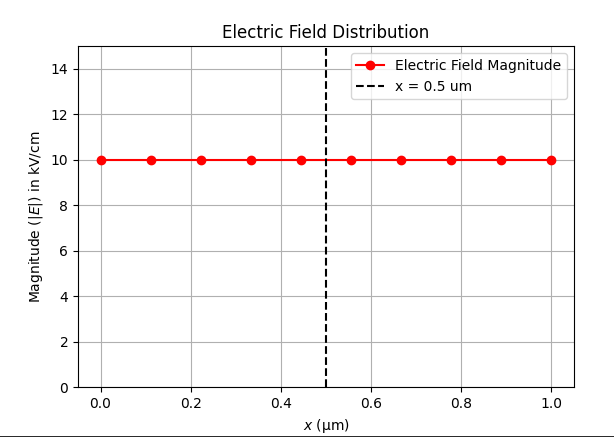
\includegraphics[width=0.4\textwidth]{grap4.png} 
        \captionof{figure}{Uniform Electric Field Magnitude of 10 kV/cm.}
    \end{minipage}
\end{center}
\vspace{0.5cm}

\section{Step 5: Final Result}
The magnitude at $x = 0.5$ $\mu$m is \textbf{10 kV/cm}.

\textbf{Correct Option: (C)}

\end{document}
